\chapter{引言}\label{chap:introduction}
近几十年来, 弹性波散射问题及其反问题在工程领域和数学领域都得到了广泛研究\cite{landau}。 特别地, 弹性波反散射问题在地球物理领域、石油勘探领域中发展迅速。
弹性波反散射问题是利用接受到的弹性波散射数据去决定障碍物的位置、形状、大小。 相比于声波, 弹性波是由横波和纵波耦合而成的矢量波, 因此研究难度更大。 又因为反问题普遍具有强非线性及高度不适定性, 这导致弹性波反散射问题的研究更具挑战性和吸引力。目前,在数学领域,学者们主要研究的弹性波反散射问题为全空间背景下的弹性波反散射问题\cite{bonnet2005inverse,bao2018inverse}和粗糙表面的弹性波反散射问题\cite{liu2019near}。 而全空间背景下的弹性波反散射问题有反障碍物问题和反源问题; 粗糙表面的弹性波反散射问题又有局部粗糙面和无穷粗糙面两种。另一方面,在勘探地球物理领域, 弹性波是在地表以下传播的, 这是一个半空间模型。于是,本文将联系实际,以数学的角度针对半空间弹性波散射问题和反散射问题加以研究,特别是考虑如何从数值上构造一个高效稳定的算法来重构障碍物。特别的,该直接成像法是基于逆时偏移的思想,且不需要障碍物是否可穿透以及其不可穿透时边界条件的先验信息。
\section{研究背景}
 散射理论研究在二十世纪的数学物理学界占据了非常重要的地位。通俗地讲, 弹性波的散射问题, 就是研究当入射波(地震源、可控震源)从一种弹性介质进入另一只弹性介质或是碰到障碍物 (散射体) 时产生的效应。 与声波、电磁波散射问题提法类似, 弹性波散射问题只是把控制方程换成了 Navier 方程。特别地, 如果我们把弹性波总场 $u(x)$ 看作是入射波 $u^i(x)$ 和散射波 $u^s(x)$的和,那么正散射问题就是根据入射波 $u^i(x)$、障碍物的物理特性以及弹性波方程去决定散射波 $u^s(x)$。 而我们本文更感兴趣的反散射问题就是利用散射波$u^s(x)$ 或是 $u^s(x)$ 在无穷远处的渐进形式来重构障碍物的位置、大小、形状。而在研究反散射问题前, 对正散射问题有一个清晰的理解是必不可少的。因此, 在后文中, 我们先来研究半空间弹性波正散射问题。
\section{弹性波半空间散射与逆散射问题}
由于地球是一个弹性体, 所以我们可以将地下看成是一个填充弹性介质的半空间。而弹性波的传播主要是用弹性波方程描述的。本文, 我们重点研究二维半空间弹性波散射问题与反散射问题。 令 x 为半空间中的一个质点, 即 
\ben
x:=(x_1,x_2)^T\in\R^2_+:=\{(y_1,y_2)^T\in\R^2:y_2>0\}
\een
令 $u(x):=(u_1(x),u_2(x))\in\C^2 $ 为在 x 处的位移。 假设弹性介质是线性各项同性均匀介质, 其 {Lam\'{e}} 常数 $\lambda$ 和 $\mu$ 满足 $\lam>0,\mu>0$, 密度函数为 $\rho$, 角频率为 $\omega>0$, 则位移函数满足如下弹性波方程:
\ben
\nabla\cdot\sigma(u(x)) +\om^2 u(x)=f(x)
\een
这里 $f(x)$ 是点x 处的外力,应力张量 $\sigma(u)\in \C^{2\times2}$ 是2阶张量, 它与应变张量 $\ep(u)\in \C^{2\times2}$ 一起满足如下本构关系 (胡克定律):
\ben
& &\sigma(u) = 2\mu\ep(u) + \lambda\div u\, \I, \\ 
& & \ep(u)=\frac{1}{2}(\na u +(\na u)^T).
\een
这里 $\I\in\R^{2\times 2}$ 是二阶恒等矩阵,$\nabla u$ 是位移梯度张量,其每个元素为 
\ben
(\na u)_{ij}=\pa u_i(x)/\pa x_j \ \ .
\een 
为了表述简便, 我们在后文中都不失一般性地假设背景介质的密度有 $\rho=1$。定义弹性波算子 
\ben
& &\Delta_e u:=(\lambda+\mu)\nabla\div \ u+\mu\Delta u
\een
易得 $\Delta_e u(x) = \nabla\cdot \sigma(u(x))$。
于是, 弹性波 u(x) 满足如下弹性波方程: 
\be
& &\Delta_e u(x)+ \rho\,\omega^2u(x)= -f 
\ee
由于弹性波在地表满足自由表面边界条件 \cite{ela_reverse,grant1965interpretation}, 即法向应力为零。有了如上表述,下面我们可以来提半空间弹性波散射问题。 假设障碍物 $D\subset\R^2_+$ 嵌入在半空间中, 且为有界 Lipschitz 区域。在本文中, 我们具体考虑不可穿透障碍物满足 Dirichlet 边界条件, 至于不可穿透情形或是可穿透情形下其它边界条件可以类似地被叙述。 进一步, 我们假设入射波是由$x_s$ 处的点源沿着 极化方向 $q\in R^2$ 激发, 于是相对应的弹性波总场 $u_q(x,x_s)$ 满足如下半空间弹性波方程: 
\be\label{eq0}
& &\Delta_e u_q(x,x_s)+ \omega^2u_q(x,x_s)= -\delta_{x_s}(x)\ \ \ \ \mbox{in }\ \ \ \R_+^2\bks \bar{D},\\ \label{eq1}
& &u_q(x,x_s)=0 \ \ \mbox{on} \ \Ga_D,\  \\
& & \sigma(u_q(x,x_s))e_2=0 \ \ \mbox{on} \ \Ga_0, \label{eq2}
\ee
这里 $\Ga_D$ 表示障碍物的表面,且令其外单位法向为 $\nu(x)$, 
\ben
\Ga_0=\{(x_1,x_2)^T\in\R^2:x_2=0\}
\een
 为半空间 $\R^2_+$ 的表面, $e_i$ 为沿着 $x_i$ 轴的单位向量, $i=1,2$。特别地, 若障碍物满足 Neumann 边界条件, 则将式 (\ref{eq1}) 替换成:
 \ben
 & &\sigma(u_q(x,x_s))\cdot\nu(x)=0 \ \ \mbox{on} \  \ \ \ \Ga_D,
 \een
若障碍物满足阻抗边界条件, 则将式 (\ref{eq1}) 替换成:
\ben
& &\sigma(u_q(x,x_s))\cdot\nu(x)+\i\eta(x)u_q(x,x_s)=0 \ \ \mbox{on} \  \ \ \ \Ga_D,
\een
这里在 $\Ga_D$ 上 $\eta\in L^\infty(\Ga_D)$ 以及 $\eta> 0$。若障碍物 $D$ 是可穿透的, 则将式 (\ref{eq0})-(\ref{eq1}) 替换成
\ben
& &\Delta_e u_q(x,x_s)+ \omega^2n(x)u_q(x,x_s)= -\delta_{x_s}(x)\ \ \ \ \mbox{in } \ \ \ \R_+^2
\een
这里 $n(x)\in L^{\infty}({\R^2_+})$ 是正函数,且当 $x\notin D$ 时,$n(x)==1$。

令 $\N(x,y)$ 为半空间中弹性波方程的 Green 函数且在 $\Ga_0$ 上满足自由边界条件 (Neumann 边界条件) ,其中 $\N(x,y)q$ 满足如下方程
\ben
& & \Delta_e [\N(x;y)q] + \omega^2 [\N(x,y)q] = -\mathbf{\delta}_y(x) q \ \ \mbox{in }\R^2_+ , \\
& & \sigma(\N(x,y)q)e_2 = 0 \ \ \mbox{on } \Gamma_0, 
\een
为了简便起见, 后文中统一称 $\N(x,y)$ 为半空间弹性波 Neumann Green 函数。令入射场 $u^i_q(x,x_s)=\N(x,x_s)q$, 于是散射场  $u^s_q(x_r,x_s)=u_q(x_r,x_s)-\N(x_r,x_s)q, x_r\in\Ga_0$,满足如下方程
\be
& &\Delta_e u_q^s(x,x_s)+ \omega^2u_q^s(x,x_s)= 0 \ \ \ \ \mbox{in }\R_+^2\bks \bar{D},\label{ep1}\\
& &u^s_q(x,x_s)=-\N(x,x_s)q \ \ \mbox{on} \ \Ga_D,\\
& & \sigma(u_q^s(x,x_s))e_2=0 \ \ \mbox{on} \ \Ga_0,\label{ep2}
\ee
为了保证方程 (\ref{p1})-(\ref{p2}) 的适定性, 一般的做法是在无穷远处方程需要满足某种边界条件或是辐射条件来保证散射波是外行波 (outgoing wave)。 通常在全空间散射问题中,散射场 $u^s(x)$ 通过 Helmholtz分解可以分成横波 $u^s_s$ 及纵波 $u^s_p$ , 且有
\ben
& &u^s_s=\frac{1}{k_s^2}\nabla\times\nabla\times u^s \\
& &u^s_p=-\frac{1}{k_p^2}\nabla\nabla\cdot u^s
\een
且在全空间中除障碍物 $D$ 以外各自满足如下方程:
\ben
& &\Delta u^s_s + k_s^2 u^s_s=0  \ \ \ \ \ \ \ \ \ \ \  \ \ \ \ \ \ \ \mbox{in} \ \  \R^2\bks\bar{D}\\
& &\Delta u^s_p + k_s^2 u^s_p =0 \ \ \ \ \ \ \ \ \ \ \  \ \ \ \ \ \ \ \mbox{in} \ \  \R^2\bks\bar{D}
\een
这里 $k_s$ 为横波波数, $k_p$ 为纵波波数, 且有
\ben
k_s=\frac{\om}{\sqrt{\mu}}=\frac{\om}{c_s}, \ \ \ \ \  k_p=\frac{\om}{\sqrt{\lambda+2\mu}}=\frac{\om}{c_p}
\een
其中  $c_s$, $c_p$ 分别为横波波速和纵波波速。 这里的旋度算子, 针对标量函数 $w(x)$, 有 
\ben
\nabla\times w(x)=(\pa_{x_2}w(x),-\pa_{x_1}w(x))^T
\een
针对二维矢量函数 $\mathbf{v}(x)=(v_1(x),v_2(x))^T$, 有
\ben
\nabla\times \mathbf{v}(x)=\pa_{x_1}v_2(x)-\pa_{x_2}v_1(x)
\een
在全空间情形下,要求 $u^s_q(x)$ 著名的 Kupradze’s 辐射条件 \cite{ku63,kupradze1976three}, 即要求横波 $u^s_s$,  纵波 $u^s_p$ 满足 Sommerfeld 辐射条件 \cite{sommerfeld1912greensche,colton-kress}:
\ben
& &\lim_{|x|\to\infty}|x|^{1/2}(\frac{\pa u^s_s(x)}{\pa |x|}-\i k_s u^s_s(x))=0, \ \\
& &\lim_{|x|\to\infty}|x|^{1/2}(\frac{\pa u^s_p(x)}{\pa |x|}-\i k_p u^s_p(x))=0
\een
在该辐射条件下, 全空间弹性波散射问题的适定性已经得到了完善的研究\cite{ku63,cxz2016,bramble2008note}。Kupradze's 辐射条件保证了弹性波在全空间中是向外传播, 而排出了内行波, 利用 Rellich 引理的推广 \cite{rellich1943über,colton-kress}, 可以证明在全空间情形下散射解的唯一性。而关于存在性, 在文献 \cite{ku63} 中, 作者针对光滑散射体给出了证明。针对 Lipschitz 边间, Bramble 和 Pasciak \cite{bramble2008note} 针对 Dirichlet 边界条件给出了证明了。针对 Neumann 边界条件, Chen 等利用极限吸收原理证明了全空间弹性波散射问题解的适定性,这对我们研究半空间弹性波散射问题有所启发。

由于自由表面条件的存在, 导致半空间弹性波中存在 Rayleigh 表面波\cite{chaillat2014new}, Kapradze's 辐射条件不在适用。Rayleigh 表面波是一种沿着半空间表面传播, 在往半空间内部传播时指数式衰减。虽然 Sommerfeld 辐射条件\cite{colton-kress,nedelec2001acoustic} 或是 kapradze's 辐射条件能保证半空间弹性波散射问题的 解的唯一性,但是由于这种条件不能刻画 Rayleigh 表面波的传播模式,所以不能保证解的存在性。事实上,后文中证明可以看到, Rayleigh 表面波的传播波速与横波和纵波的波速也是不同的。 在文献\cite{nedelec2011}中, N{\'e}d{\'e}lec 等人通过研究半空间弹性波 Neumann Green 函数在无穷远处的渐进性质, 提出来新的弹性波辐射条件,并且在该辐射条件下作者证明了如下方程解的存在唯一性
\ben
& &\Delta_e u_q(x,x_s)+ \rho\,\omega^2u_q(x,x_s)= -\delta_{x_s}(x)\ \ \ \ \mbox{in }\R_+^2,\\
& & \sigma(u_q(x,x_s))e_2=f\ \  \ \ \ \ \ \mbox{on} \ \Ga_0,
\een
其中应力源 $f$ 在$\Ga_0$ 上存在紧支集。

 在文献 \cite{arens2001uniqueness,arens2002existence}中,Arens 针对固支边界 (clamped or rigid boundary) 的粗糙表面弹性波散射问题, 提出来上行辐射条件(upwards propagating radiation conditon)。 该辐射条件给出了一种显式的 Dirichlet-to-Neumann 映射, 可以用来将无穷的半空间截断成包含粗糙表面的条状空间。而 Charalambopolos, Gintides 和 Kiriaki \cite{charalambopoulos2002radiation} 利用了角谱表示法作为散射条件, 将 Arens \cite{arens2001uniqueness} 的工作推广到自由表面情形, 但是该文章缺少严格的数学证明。
 
 进一步的,针对满足自由表面边界条件的半空间层状介质, Alem 和 Chorfi \cite{alem2003theoreme} 给出了一个有趣的方法。 他们的散射条件不在作用于单独的横波和纵波,而是描述混合波的法向应力和位移在无穷远处的关系, 有点类似与 N{\'e}d{\'e}lec \cite{nedelec2011} 中的辐射条件。 该辐射条件的好处是类似于声波中的 Sommerfeld 辐射条件, 它可以很好地适用于与弹性波中的积分公式 (Betti's 公式 \cite{ku63})的整合。然而,作者还强行施加了一个无穷远处的衰减条件 $\mathbf{O}(1/R)$, 此时 Rayleigh 表面波无法满足此条件。
 
 类似与声波中,全局积分辐射条件\cite{colton-kress}与 Sommefeld 辐射条件等价, Madyarov 和 Guzina \cite{Guzina2006} 将辐射条件表示成在一个半径足够大的半圆上的积分的极限,而不同于局部散射条件是表示成函数与其导数间组合的极限。
 \ben
 	\lim_{r\to\infty}  \int_{S_r^+} (\sigma(\N(x,y)e_i)\hat{r})\cdot u(x) - (\N(x,y)e_i)\cdot (\sigma(u)\hat{r})ds(x)=0
 \een
 这里 $S_r^+:=\{x\in \R^2_+ \ | \ \|x\|=r^2\}$, $\hat{r}=x/r$ 和 $y\in \R_+^2$。  该辐射条件需要用到满足相应半空间表面边界条件的 Green 函数, 其好处是可以直接得到散射波在障碍物表面的积分表示。然而该文章在证明散射解的唯一性前假设了解的存在性。
 
 在本文中, 我们不再针对半空间弹性波障碍物散射问题来研究相应的散射条件。我们受文献 \cite{Yves1988,wilcox1975,leis}的启发, 将利用极限吸收原理来定义半空间弹性波散射问题的解。 具体地, 我们考虑$u^s_{q,\ep}$ 是满足角频率为 $\om(1+\i\ep)$ 的半空间弹性波方程,即为
 \ben
 & &\Delta_e u_{q,\ep}^s(x,x_s)+ \omega^2(1+\i\ep)^2 u_{q,\ep}^s(x,x_s)= 0 \ \ \ \ \mbox{in }\R_+^2\bks \bar{D},\label{p12}\\
 & &u^s_{q,\ep}(x,x_s)=-\N(x,x_s)q \ \ \ \ \ \mbox{on} \ \ \ \ \Ga_D,\\
 & & \sigma(u_{q,\ep}^s(x,x_s))e_2=0 \ \ \ \ \ \mbox{on} \ \ \ \ \ \ \ \Ga_0,\label{p22}
 \een
  于是, 方程(\ref{ep1})-(\ref{ep2}) 中的散射解 $u_q^s(x,x_s)$ 定义为 $u_{q,\ep}^s(x,x_s)$ 在 $\ep\to 0^+$ 时某种范数意义下极限,我们将在第 \ref{chap:Elastic} 章中做详细讨论。
 
 

\begin{figure}[htbp]
	\centering
	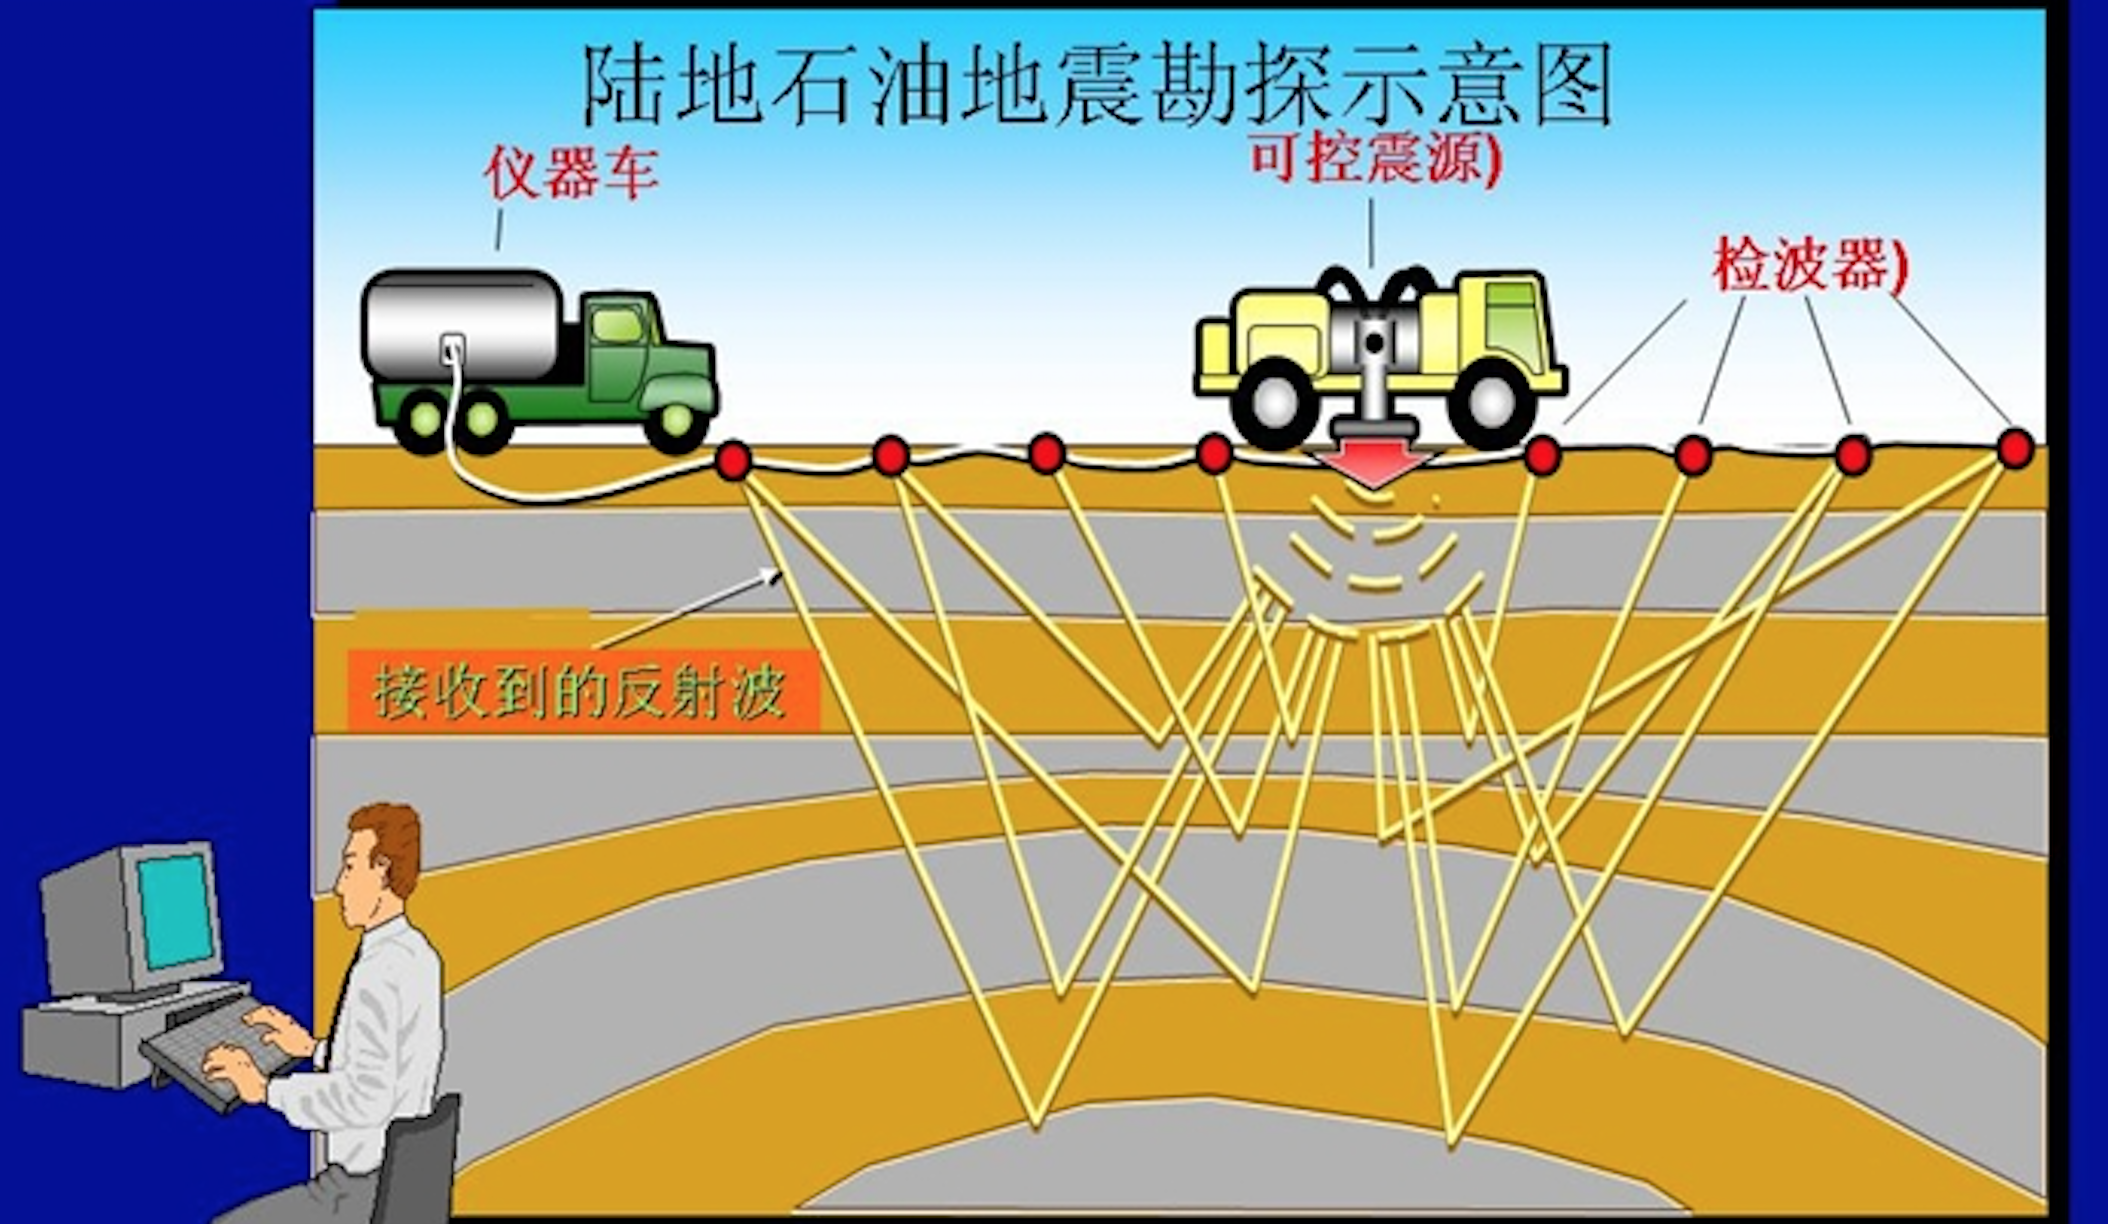
\includegraphics[width=\textwidth]{./Img/seismic2}
	\caption{地震波勘探模型} \label{figure_seismic}
\end{figure}

本文主要对上述半空间弹性波散射问题的反障碍物问题感兴趣。我们在远离障碍物的接受点 $x_r$ 上测量数据 $u^s_q(x_r,x_s)$。 然后, 我们通过接受到的数据来重构出障碍物的位置、大小、形状。	特别地,由地震勘探模型启发 (如图\ref{figure_seismic}), 我们假设发射点和接收点都在半空间表面, 即 $x_s\in\Ga_0$, $x_r\in \Ga_0$。其中, 为了使式子 (\ref{eq0}) 中的源项 $\delta_{x_s}(x)$ 有意义, 我们这里将 $x_s\in\Ga_0$ 看作是 $x_s\in\R^2_+\bks\bar{D}$ 趋向于 $\Ga_0$ 的极限。

由于反问题是高度线性不适定问题 \cite{hadamard1923lectures}, 换言之, 如果我们测量到的数据不准确或是有一个微小的扰动, 都会可能导致相对应的障碍物带来巨大的误差。




\section{逆时偏移法简介}
\section{本文的研究成果}
